\chapter{Numerical Results}\label{sec:numerical_results}

This chapter presents the results of the numerical experiments conducted to
study the behavioural patterns that can emerge from the interaction between the
two EDs and the EMS.
This chapter consists of a \textit{Data Collection} section, which describes the
data collection process, and a \textit{What if scenarios} section, which
presents the results of the numerical experiments.
Note that the data presented in this chapter are archived and can be found
in~\cite{michalis_panayides_2023_7501988}.


\section{Data Collection}\label{sec:data_collection}

The data presented in this chapter were collected by solving the game theoretic
model from the interaction of the two EDs and the EMS.
Essentially, the collected data are the matrices \(A, B\) and \(R\) described
in Section~\ref{sec:queueing_systems_and_normal_form_games}.
Each triplet of matrices \((A, B, R)\) was generated by solving the
corresponding game for a different set of parameters.

Different values of the parameters were used to generate this dataset.
The parameters that were changed throughout these experiments are listed in
Table~\ref{tab:data_collection_parameters}.

\begin{table}[H]
    \centering
    \caption{Data collection: Parameters}
    \begin{tabular}{|c|c|}
        \hline
        Parameter & Description \\
        \hline
        \(\lambda_2\) & Arrival rate of patients in EMS \\
        \(\alpha\) & Weight of lost individuals over time blocked \\
        \(t\) & Time target for the EDs \\
        \(\lambda_1^A\) & Arrival rate of patients in ED \(A\) \\
        \(\lambda_1^B\) & Arrival rate of patients in ED \(B\) \\
        \(\mu^A\) & Service rate of patients in ED \(A\) \\
        \(\mu^B\) & Service rate of patients in ED \(B\) \\
        \(C^A\) & Number of servers in ED \(A\) \\
        \(C^B\) & Number of servers in ED \(B\) \\
        \(N^A\) & Maximum capacity in ED \(A\) \\
        \(N^B\) & Maximum capacity in ED \(B\) \\
        \(M^A\) & Maximum capacity of parking space in ED \(A\) \\
        \(M^B\) & Maximum capacity of parking space in ED \(B\) \\
        \hline
    \end{tabular}
    \label{tab:data_collection_parameters}
\end{table}

A python script was ran that iterates over different values of the parameters.
Overall, \(5160404\) different sets of parameters were used.
For each parameter set, the script solves the game and stores the resulting
entries of the matrices \((A, B, R)\) as well as the parameters used to generate
them in sub-directory of the \lstinline{data} directory.
All parameter values of each parameter set, along with the corresponding values
of \(A, B\) and \(R\), are mapped to a unique fixed-size hash value which is
used as the name of the sub-directory for that parameter set.
The hash function that is used for this operation is the MD5 message-digest
algorithm~\cite{rivest1992md5}.

Having the name of the sub-directory for the current parameter set, the
resulting matrices are stored in a compressed \lstinline{.npz} file in that
sub-directory.
The \lstinline{.npz} file format is a zipped archive of files
named after the variables they contain, which are stored using numpy's
\lstinline[style=pystyle]{savez_compressed} function~\cite{2020NumPy-Array}.
The \lstinline{.npz} files can be loaded using numpy's
\lstinline[style=pystyle]{load} function.
In addition, to the \lstinline{.npz} file, a
\lstinline{README.md} file containing general instructions and a
\lstinline{.csv} file containing the value of each parameter is
also stored in each sub-directory.
The following code snippet shows an example of how the data are stored and
loaded using numpy.

% TODO: Somehow remove np.savez_compressed from doctesting
\begin{lstlisting}[style=pystyle]
>>> import numpy as np
>>> array_1, array_2 = np.arange(10), np.arange(10, 20)
>>> np.savez_compressed("demo", array_1=array_1, array_2=array_2)
>>> loaded_file = np.load("demo.npz")
>>> loaded_file["array_1"]
array([0, 1, 2, 3, 4, 5, 6, 7, 8, 9])
>>> loaded_file["array_2"]
array([10, 11, 12, 13, 14, 15, 16, 17, 18, 19])

\end{lstlisting}

Apart from every sub-directory containing the data for a specific parameter set,
there is also a sub-directory named \lstinline{_parameters}.
This sub-directory contains a \lstinline{.csv} file containing the
values of all parameters used in the experiments along with their corresponding
hash values.
This file can be used to map the hash values of the sub-directories to the
corresponding parameter values.
Consider the first \(5\) entries of the \lstinline{.csv} file
from the \lstinline{_parameters} sub-directory and the first
\(5\) directories in the \lstinline{data} directory.

\begin{table}[H]
    \centering
    \caption{Contents of \lstinline{_parameters/main.csv} file}
    \begin{tabular}{|cccccccccccccl|}
        \hline
        0 & 5 & 4 & 0 & 0 & 0.1 & 2 & 3 & 3 & 2 & 6 & 7 & 0 &
        0c2d6a2e23de39d69ffb3b2a18d33692 \\
        0 & 5 & 4 & 0 & 0 & 0.1 & 2 & 3 & 3 & 2 & 6 & 7 & 1 &
        8268e1967541e5d8edff3f3f00a4cfb8 \\
        0 & 5 & 4 & 0 & 0 & 0.1 & 2 & 3 & 3 & 2 & 6 & 7 & 2 &
        95d86d6bdca819eff8acc3d7a9297fd5 \\
        0 & 5 & 4 & 0 & 0 & 0.1 & 2 & 3 & 3 & 2 & 6 & 7 & 3 &
        b60ba099d5eabf6f07a9d9a81a2bab59 \\
        0 & 5 & 4 & 0 & 0 & 0.1 & 2 & 3 & 3 & 2 & 6 & 7 & 4 &
        2f542f3e30736267ace3bb24a45de427 \\
        \hline
    \end{tabular}
    \label{tab:parameters_csv}
\end{table}

The corresponding sub-directories of the \lstinline{data}
directory are shown in the tree structure in Figure~\ref{fig:data_directory}:

\begin{figure}[H]
    \dirtree{%
        .1 data.
        .2 0c2d6a2e23de39d69ffb3b2a18d33692.
        .3 main.csv.
        .3 main.npz.
        .3 README.md.
        .2 8268e1967541e5d8edff3f3f00a4cfb8.
        .3 main.csv.
        .3 main.npz.
        .3 README.md.
        .2 95d86d6bdca819eff8acc3d7a9297fd5.
        .3 main.csv.
        .3 main.npz.
        .3 README.md.
        .2 b60ba099d5eabf6f07a9d9a81a2bab59.
        .3 main.csv.
        .3 main.npz.
        .3 README.md.
        .2 2f542f3e30736267ace3bb24a45de427.
        .3 main.csv.
        .3 main.npz.
        .3 README.md.
    }
    \caption{Structure of the \lstinline{data} directory}
    \label{fig:data_directory}
\end{figure}
    
The \lstinline{main.csv} file in each sub-directory contains the values of the
parameters used to generate the data in that sub-directory.
The \lstinline{main.npz} file contains the compressed entries of the matrices
\(A, B\) and \(R\).
The complete dataset is archived using \url{www.zenodo.org} and can be found
with the following DOI:
\url{10.5281/zenodo.7501988}~\cite{michalis_panayides_2023_7501988}.


\section{Dataset description}\label{sec:dataset_description}

As mentioned in Section~\ref{sec:data_collection}, the dataset contains
matrices \(A, B\) and \(R\) for a total of \(5,160,404\) parameter sets.
A descriptive analysis of the values of the parameters used in the experiments
is shown in Table~\ref{tab:parameters_descriptive}.


\begin{table}[H]
    \centering
    \caption{Descriptive statistics of the dataset}
    \begin{tabular}{|c|cccc|}
        \hline
        Parameter & Mean & Standard Deviation & Minimum & Maximum \\
        \hline
        \(\lambda_2\) & 4.545320 & 7.045888 & 0.100000 & 161.821844 \\
        \(\alpha\) & 0.504179 & 0.305070 & 0.000000 & 1.000000 \\
        \(t\) & 4.999915 & 3.036935 & 0.000000 & 10.000000 \\
        \hline
        \(\lambda_1^B\) & 1.217896 & 2.050153 & 0.000000 & 34.019111 \\
        \(\mu^A\) & 2.024239 & 0.400677 & 0.420571 & 6.773554 \\
        \(C^A\) & 1.081755 & 0.680075 & 1.000000 & 9.000000 \\
        \(N^A\) & 2.107661 & 0.821679 & 2.000000 & 24.000000 \\
        \(M^A\) & 2.045482 & 0.456713 & 1.000000 & 20.000000 \\
        \hline
        \(\lambda_1^A\) & 1.156440 & 2.628927 & 0.000000 & 60.961985 \\
        \(\mu^B\) & 2.052536 & 0.421094 & 2.000000 & 6.602015 \\
        \(C^B\) & 1.102124 & 0.784007 & 1.000000 & 9.000000 \\
        \(N^B\) & 2.121707 & 0.804273 & 2.000000 & 28.000000 \\
        \(M^B\) & 2.071752 & 0.560980 & 2.000000 & 16.000000 \\
        \hline
    \end{tabular}
    \label{tab:parameters_descriptive}
\end{table}


Not all values listed in Table~\ref{tab:parameters_descriptive} are used equally
often.
In fact consider the values of the parameter \(\lambda_2\) that range from
\(0.1\) to \(162\).
Figure~\ref{fig:data_description_lambda_2} shows the number of times each
value of \(\lambda_2\) is used in the dataset.

\begin{figure}[H]
    \centering
    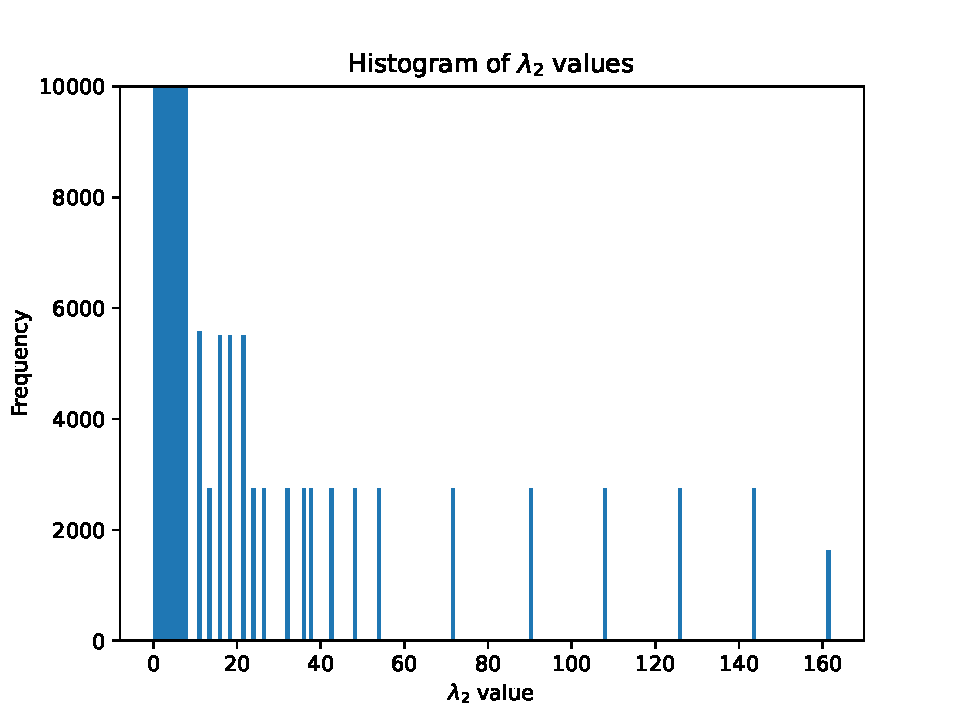
\includegraphics[width=\linewidth]{chapters/05_numerical_results/Bin/lambda_2_histogram.pdf}
    \caption{Number of times each value of \(\lambda_2\) is used in the dataset}
    \label{fig:data_description_lambda_2}
\end{figure}

It can be seen that the values of \(\lambda_2\) that are used the most are
the ones from \(0.1\) to \(10\).
In fact, the y-axis of Figure~\ref{fig:data_description_lambda_2} has been cut
at \(10,000\) to better show the values of \(\lambda_2\) that are greater than
\(10\).
Figure~\ref{fig:data_description_lambda_2_0_10} shows the zoomed-in version of
Figure~\ref{fig:data_description_lambda_2} where only values of \(\lambda_2\)
from \(0\) to \(10\) are shown.
From Figures~\ref{fig:data_description_lambda_2}
and~\ref{fig:data_description_lambda_2_0_10} it can be seen that the values of
\(\lambda_2\) that are used the most are the ones from \(0\) to \(10\).

\begin{figure}[H]
    \centering
    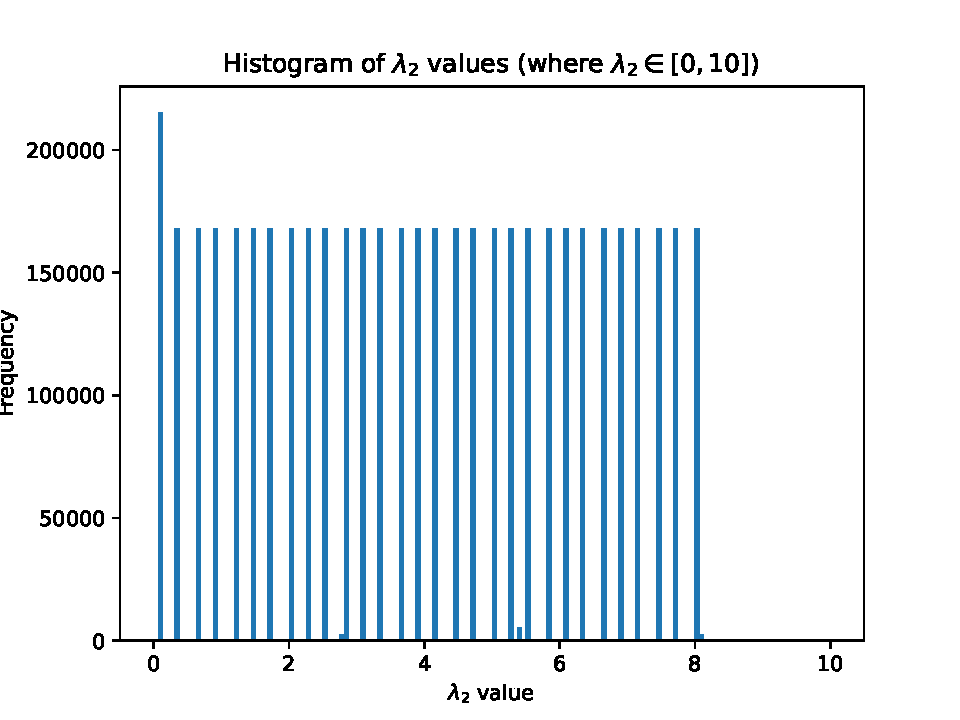
\includegraphics[width=\linewidth]{chapters/05_numerical_results/Bin/lambda_2_histogram_0_10.pdf}
    \caption{Number of times each value of \(\lambda_2\) is used in the dataset
        for \(\lambda_2 \in [0, 10]\)}
    \label{fig:data_description_lambda_2_0_10}
\end{figure}

In addition, in terms of the values of \(C, N\) and \(M\) of the two players
\(A\) and \(B\), only some combinations of these values were explored.
Figures~\ref{fig:parameter_space_C_N_M_A} and~\ref{fig:parameter_space_C_N_M_B}
show the explored combinations of the values of \(C, N\) and \(M\) for player
\(A\) and player \(B\) respectively.

\begin{figure}[H]
    \centering
    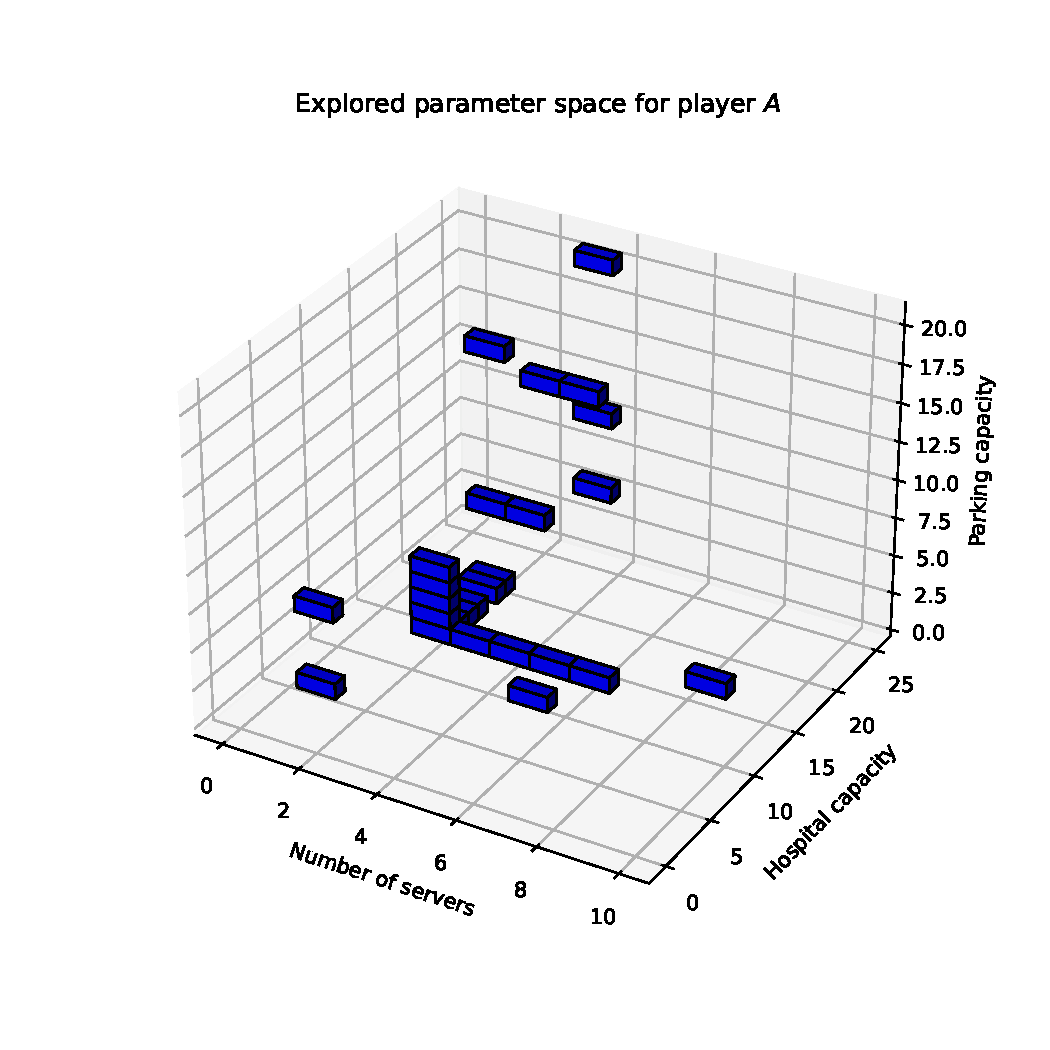
\includegraphics[width=\linewidth]{chapters/05_numerical_results/Bin/explored_parameters_1.pdf}
    \caption{Explored combinations of the values of \(C, N\) and \(M\) for
    player \(A\)}
    \label{fig:parameter_space_C_N_M_A}
\end{figure}

\begin{figure}[H]
    \centering
    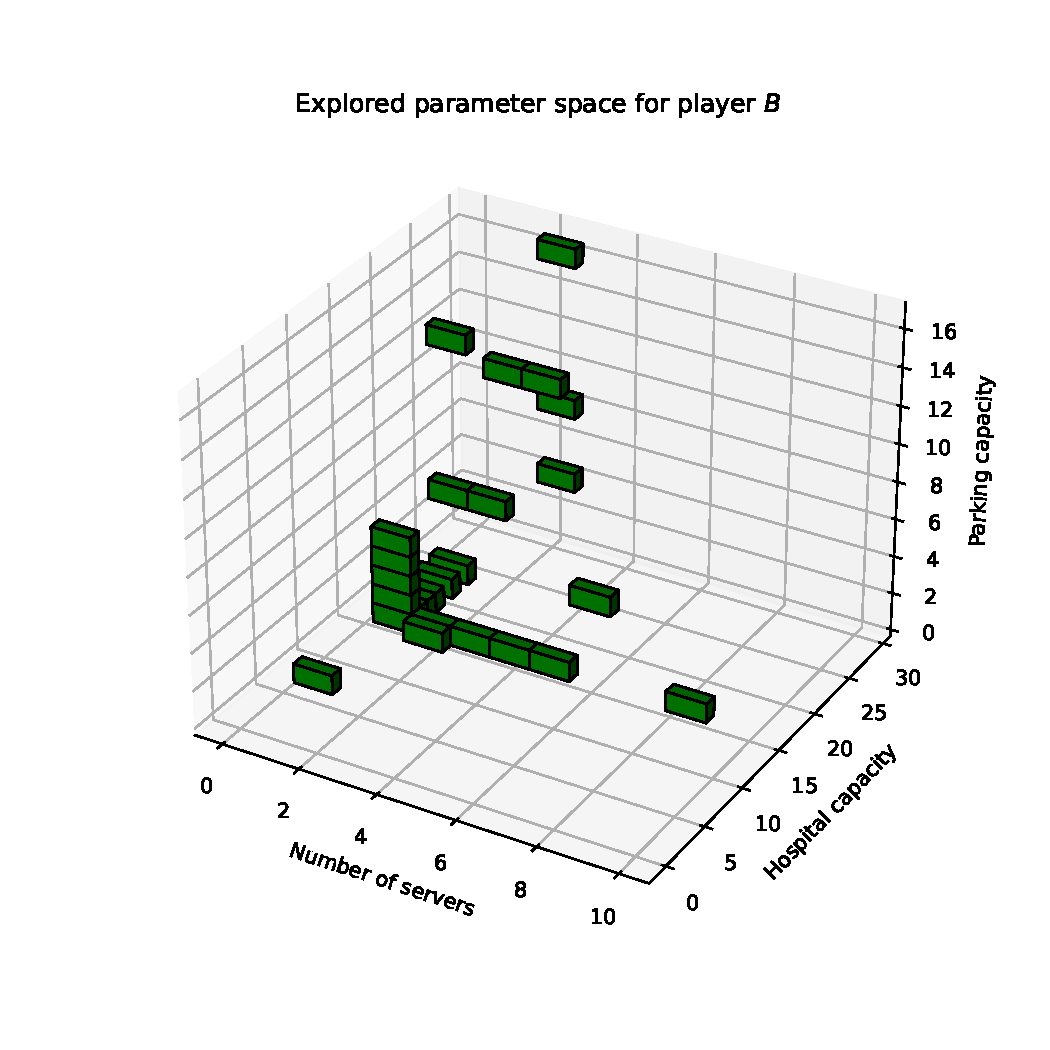
\includegraphics[width=\linewidth]{chapters/05_numerical_results/Bin/explored_parameters_2.pdf}
    \caption{Explored combinations of the values of \(C, N\) and \(M\) for
    player \(B\)}
    \label{fig:parameter_space_C_N_M_B}
\end{figure}

From Figures~\ref{fig:parameter_space_C_N_M_A}
and~\ref{fig:parameter_space_C_N_M_B} it can be seen that only a small subset
of the possible combinations of the values of \(C, N\) and \(M\) were explored.
Note here that for each of this explored combinations additional combinations
of the values of \(\lambda_2, \lambda_1^A, \lambda_1^B, \mu^A, \mu^B, \alpha\)
and \(t\) were also used.


\section{What if scenarios}\label{sec:results_what_if}

